\documentclass[a4paper,12pt]{article}
\usepackage{standalone}
\usepackage[a4paper, top=0.8in, bottom=0.7in, left=0.8in, right=0.8in]{geometry}
\usepackage{amsmath}
\usepackage{hyperref}
\usepackage{amsfonts}
\usepackage{latexsym}
\usepackage{graphicx}
\usepackage{fancyhdr}
\usepackage{enumitem}
\usepackage{setspace}
\usepackage{tcolorbox}
\usepackage{tikz}
\usepackage{multicol}
\usepackage[defaultfam,tabular,lining]{montserrat} % Font settings for Montserrat

\sloppy

\title{}
\date{}
\hyphenpenalty=10000
\exhyphenpenalty=10000

\setlength{\parindent}{0pt}
\pagestyle{fancy}

\setlength{\headheight}{27.11148pt}
\addtolength{\topmargin}{-15.11148pt}

\fancyhf{}
\fancyhead[L]{\textbf{Curriculum F SWB}}
\fancyhead[R]{
\includegraphics[width=0.8cm]{Round Logo.png}} % Placeholder for logo
\fancyfoot[C]{\footnotesize \textcopyright{} Study Smart Tutors}

\sloppy

% Define a new command for the level letter
\newcommand{\levelLetter}{F}  % Change this letter to update throughout the document

%%%%%%%%%%%%%%%%%%%%%%%%%%%%%%%%%%%%%

\begin{document}

% Title Page
\documentclass[12pt]{article}
\usepackage[a4paper, top=0.8in, bottom=0.7in, left=0.8in, right=0.8in]{geometry}
\usepackage{amsmath}
\usepackage{amsfonts}
\usepackage{latexsym}
\usepackage{graphicx}
\usepackage{tikz}
\usepackage{fancyhdr}
\usepackage{tcolorbox}
\usepackage{multicol}
\usepackage{tgadventor}
\renewcommand{\familydefault}{\sfdefault}
\usepackage{enumitem}
\usepackage{setspace}
\setlength{\parindent}{0pt}
\pagestyle{fancy}
\usepackage{needspace}


% Define a new command for the level letter
\newcommand{\levelLetter}{F}  % Change this letter to update throughout the document

%%%%%%%%%%%%%%%%%%%%%%%%%%%%%%%%%%%%%

\setlength{\headheight}{27.11148pt}
\addtolength{\topmargin}{-15.11148pt}

\fancyhf{}
%\fancyhead[L]{\textbf{5.NBT.A.1: Understand the Place Value System}}
\fancyhead[R]{
\includegraphics[width=0.8cm]{Round Logo.png}}
\fancyfoot[C]{\footnotesize © Study Smart Tutors}






\title{}
\date{}
\hyphenpenalty=10000
\exhyphenpenalty=10000

\begin{document}


% COVER PAGE 1 BEGIN
% Skip header and footer on the first page
\thispagestyle{empty}

% Vertical centering
\vspace*{\fill}

\vspace*{3cm}

\begin{center}

    % Logo
    
\includegraphics[width=0.6\textwidth]{SST_Color_Logo.png} % Replace 'logo.png' with the path to your logo file
    
    \vspace{1cm} % Space between logo and title
    
    % Cycle Name
    \Huge \textbf{} \\
    \vspace{0.2cm}
    
    % Assessment Title
    \Huge \textbf{Mathematics Tutoring}\\ 
     \vspace{1 cm}
      \LARGE \textit{Curriculum \levelLetter}\\[1cm]
 \vspace{0.5cm}
    
   


     % Name Field
    \LARGE \textbf{Name:} \underline{\hspace{8cm}}

    
    \vfill % Push the footer to the bottom
    
\end{center}


\newpage
\thispagestyle{empty}
\vspace*{\fill}
\newpage


\newpage


% STUDENT COVER PAGE  COMPLETE


\end{document}
 % Include the title page content here

% Table of Contents
\tableofcontents
\newpage

% Guided Lesson and Problem Set for 5.NR.1.1, 5.NR.1.2
\newpage
\section{5.NR.1.1, 5.NR.1.2 Guided Lesson}
\documentclass[12pt]{article}
\usepackage[a4paper, top=0.8in, bottom=0.7in, left=0.8in, right=0.8in]{geometry}
\usepackage{amsmath}
\usepackage{amsfonts}
\usepackage{latexsym}
\usepackage{graphicx}
\usepackage{fancyhdr}
\usepackage{tcolorbox}
\usepackage{enumitem}
\usepackage{setspace}
\usepackage[defaultfam,tabular,lining]{montserrat} % Font settings for Montserrat

% ChatGPT Directions:
% ----------------------------------------------------------------------
% This template is designed for creating guided lessons that align strictly with specific standards.
% Key points to ensure proper usage:
% 
% 1. **Key Concepts and Vocabulary**:
%    - Include only the concepts necessary for meeting the standards.
%    - Each Key Concept section must align explicitly with the standards being addressed.
%    - If unrelated standards are introduced (e.g., introducing new operations or properties),
%      create additional Key Concept sections labeled "Part 2," "Part 3," etc.
% 2. **Examples**:
%    - Provide concrete worked examples to illustrate the Key Concepts.
%    - These should directly tie back to the Key Concepts presented earlier.
% 3. **Guided Practice**:
%    - Problems should reinforce Key Concepts and Examples.
%    - Allow for ample spacing between problems to give students room for work.
% 4. **Additional Notes**:
%    - Use this section for helpful but non-essential concepts, strategies, or teacher notes.
%    - Examples: Fact families, properties of operations, or alternative explanations.
% 5. **Independent Practice**:
%    - Provide problems for students to practice Key Concepts individually.
% 6. **Exit Ticket**:
%    - Include a reflective or assessment-based question to evaluate student understanding.
% ----------------------------------------------------------------------

\setlength{\parindent}{0pt}
\pagestyle{fancy}

\setlength{\headheight}{27.11148pt}
\addtolength{\topmargin}{-15.11148pt}

\fancyhf{}
%\fancyhead[L]{\textbf{Standard(s): 5.NBT.A.1, 5.NBT.A.2}}
\fancyhead[R]{
\includegraphics[width=0.8cm]{Round Logo.png}} % Placeholder for logo
\fancyfoot[C]{\footnotesize © Study Smart Tutors}

\sloppy

\title{}
\date{}
\hyphenpenalty=10000
\exhyphenpenalty=10000

\begin{document}

\subsection*{Guided Lesson: Understanding Place Value and Patterns in Powers of 10}
\onehalfspacing

% Learning Objective Box
\begin{tcolorbox}[colframe=black!40, colback=gray!5, 
coltitle=black, colbacktitle=black!20, fonttitle=\bfseries\Large, 
title=Learning Objective, halign title=center, left=5pt, right=5pt, top=5pt, bottom=15pt]
\textbf{Objective:} Understand place value to the thousandths, explain patterns when multiplying or dividing by powers of 10, and apply this knowledge to solve real-world problems.
\end{tcolorbox}

\vspace{1em}

% Key Concepts and Vocabulary
\begin{tcolorbox}[colframe=black!60, colback=white, 
coltitle=black, colbacktitle=black!15, fonttitle=\bfseries\Large, 
title=Key Concepts and Vocabulary, halign title=center, left=10pt, right=10pt, top=10pt, bottom=15pt]
\textbf{Key Concepts:}
\begin{itemize}
    \item \textbf{Place Value Relationships:} Each place value represents 10 times the value of the place to its right. For example:
    \[
    3,456.789 = 3,000 + 400 + 50 + 6 + 0.7 + 0.08 + 0.009.
    \]
    \item \textbf{Patterns in Powers of 10:}
    \begin{itemize}
        \item Multiplying by \( 10, 100, \) or \( 1,000 \) shifts the decimal point to the right.
        \item Dividing by \( 10, 100, \) or \( 1,000 \) shifts the decimal point to the left.
    \end{itemize}
    \item \textbf{Rounding Numbers:} Rounding simplifies numbers to a specific place value. For example, rounding \( 3,456.789 \) to the nearest tenth gives \( 3,456.8 \).
\end{itemize}
\end{tcolorbox}

\vspace{1em}

% Examples Box
\begin{tcolorbox}[colframe=black!60, colback=white, 
coltitle=black, colbacktitle=black!15, fonttitle=\bfseries\Large, 
title=Examples, halign title=center, left=10pt, right=10pt, top=10pt, bottom=15pt]
\textbf{Example 1: Understanding Place Value}
\begin{itemize}
    \item Problem: What is the value of the digit \( 7 \) in \( 7,845.3 \) and \( 8.347 \)?
    \item Solution:
    \begin{itemize}
        \item In \( 7,845.3 \), \( 7 \) is in the thousand’s place, so its value is \( 7,000 \).
        \item In \( 8.347 \), \( 7 \) is in the thousandths place, so its value is \( 0.007 \).
    \end{itemize}
\end{itemize}

\textbf{Example 2: Multiplying by Powers of 10}
\begin{itemize}
    \item Problem: Multiply \( 3.45 \times 10, 100, \) and \( 1,000 \). What pattern do you notice?
    \item Solution:
    \begin{itemize}
        \item \( 3.45 \times 10 = 34.5 \) (shift decimal 1 place right).
        \item \( 3.45 \times 100 = 345 \) (shift decimal 2 places right).
        \item \( 3.45 \times 1,000 = 3,450 \) (shift decimal 3 places right).
    \end{itemize}
    Pattern: Multiplying by powers of 10 moves the decimal point to the right based on the number of zeros in the power of 10.
\end{itemize}

\textbf{Example 3: Dividing by Powers of 10}
\begin{itemize}
    \item Problem: Divide \( 5,600 \div 10, 100, \) and \( 1,000 \). What pattern do you notice?
    \item Solution:
    \begin{itemize}
        \item \( 5,600 \div 10 = 560 \) (shift decimal 1 place left).
        \item \( 5,600 \div 100 = 56 \) (shift decimal 2 places left).
        \item \( 5,600 \div 1,000 = 5.6 \) (shift decimal 3 places left).
    \end{itemize}
    Pattern: Dividing by powers of 10 moves the decimal point to the left based on the number of zeros in the power of 10.
\end{itemize}

\textbf{Example 4: Rounding Numbers}
\begin{itemize}
    \item Problem: Round \( 7,845.67 \) to the nearest hundred and the nearest tenth.
    \item Solution:
    \begin{itemize}
        \item Nearest hundred: \( 7,846 \to 7,800 \) (look at the tens digit).
        \item Nearest tenth: \( 7,845.67 \to 7,845.7 \) (look at the hundredths digit).
    \end{itemize}
\end{itemize}
\end{tcolorbox}

\vspace{1em}

% Guided Practice
\begin{tcolorbox}[colframe=black!60, colback=white, 
coltitle=black, colbacktitle=black!15, fonttitle=\bfseries\Large, 
title=Guided Practice, halign title=center, left=10pt, right=10pt, top=10pt, bottom=15pt]
\textbf{Solve the following problems with teacher support:}
\begin{enumerate}[itemsep=3em]
    \item Write \( 6,708.25 \) in expanded form.
    \item Multiply \( 4.32 \times 10, 100, \) and \( 1,000 \). Describe the pattern.
    \item Divide \( 12,450 \div 10, 100, \) and \( 1,000 \). Describe the pattern.
    \item Round \( 23,789.56 \) to the nearest thousand, hundred, and tenth.
\end{enumerate}
\end{tcolorbox}

\vspace{1em}

% Independent Practice
\begin{tcolorbox}[colframe=black!60, colback=white, 
coltitle=black, colbacktitle=black!15, fonttitle=\bfseries\Large, 
title=Independent Practice, halign title=center, left=10pt, right=10pt, top=10pt, bottom=15pt]
\textbf{Solve the following problems independently:}
\begin{enumerate}[itemsep=3em]
    \item What is the value of the digit \( 5 \) in \( 35,472.89 \)?
    \item Write \( 7,230.045 \) in expanded form.
    \item Multiply \( 0.784 \times 10, 100, \) and \( 1,000 \).
    \item Divide \( 98,340 \div 10, 100, \) and \( 1,000 \).
    \item Round \( 6,235.478 \) to the nearest hundred and nearest hundredth.
\end{enumerate}
\end{tcolorbox}

\vspace{1em}

% Exit Ticket
\begin{tcolorbox}[colframe=black!60, colback=white, 
coltitle=black, colbacktitle=black!15, fonttitle=\bfseries\Large, 
title=Exit Ticket, halign title=center, left=10pt, right=10pt, top=10pt, bottom=15pt]
\textbf{Answer the following question:}
\begin{itemize}
    \item What happens to a number when it is divided by \( 1,000 \)? Provide an example and explain the pattern.
\end{itemize}
\end{tcolorbox}

\end{document}


\newpage
\section{5.NR.1.1, 5.NR.1.2 Problem Set}
% ChatGPT Directions 0 :  
% This is a Tbox Problem set for the following standards: 5.NBT.A.1, 5.NBT.A.2 
%--------------------------------------------------
\documentclass[12pt]{article}
\usepackage[a4paper, top=0.8in, bottom=0.7in, left=0.8in, right=0.8in]{geometry}
\usepackage{amsmath}
\usepackage{amsfonts}
\usepackage{latexsym}
\usepackage{graphicx}
\usepackage{fancyhdr}
\usepackage{tcolorbox}
\usepackage{enumitem}
\usepackage{setspace}
\usepackage[defaultfam,tabular,lining]{montserrat} % Font settings for Montserrat

% General Comment: Template for creating problem sets in a structured format with headers, titles, and sections.
% This document uses Montserrat font and consistent styles for exercises, problems, and performance tasks.

% -------------------------------------------------------------------
% Directions for LaTeX Styling and Content
% 1. Include a header with standards and topic title: \fancyhead[L]{\textbf{<Standards>: <Topic Title>}}.
% 2. Section Breakdown:
%    - Learning Objective: Concise goal statement.
%    - Exercises: Procedural fluency tasks.
%    - Problems: Moderately complex scenarios.
%    - Performance Task: Real-world, multi-step tasks.
%    - Reflection: Prompt to reflect on strategies and learning.
% 3. Styling with tcolorbox:
%    - Frame color: colframe=black!60.
%    - Background color: colback=gray!5 or white.
%    - Title Background: colbacktitle=black!15.
%    - Font Style: Bold and large (fonttitle=\bfseries\Large).
% -------------------------------------------------------------------

\setlength{\parindent}{0pt}
\pagestyle{fancy}

\setlength{\headheight}{27.11148pt}
\addtolength{\topmargin}{-15.11148pt}

\fancyhf{}
%\fancyhead[L]{\textbf{5.NBT.A.1, 5.NBT.A.2: Place Value and Patterns in Powers of 10}}
\fancyhead[R]{
\includegraphics[width=0.8cm]{Round Logo.png}} % Placeholder for logo
\fancyfoot[C]{\footnotesize © Study Smart Tutors}

\sloppy

\title{}
\date{}
\hyphenpenalty=10000
\exhyphenpenalty=10000

\begin{document}

\subsection*{Problem Set: Place Value and Patterns in Powers of 10}
\onehalfspacing

% Learning Objective Box
\begin{tcolorbox}[colframe=black!40, colback=gray!5, 
coltitle=black, colbacktitle=black!20, fonttitle=\bfseries\Large, 
title=Learning Objective, halign title=center, left=5pt, right=5pt, top=5pt, bottom=15pt]
\textbf{Objective:} Understand place value to the thousandths and explain patterns when multiplying or dividing by powers of 10.
\end{tcolorbox}

% Exercises Box
\begin{tcolorbox}[colframe=black!60, colback=white, 
coltitle=black, colbacktitle=black!15, fonttitle=\bfseries\Large, 
title=Exercises, halign title=center, left=10pt, right=10pt, top=10pt, bottom=30pt]
\begin{enumerate}[itemsep=3em]
    \item Round \( 3,456.789 \) to the nearest whole number, tenth, and hundredth.
    \item What is the value of the digit \( 7 \) in \( 7,845 \)? What about in \( 7.845 \)?
    \item Multiply \( 3.45 \) by \( 10, 100, \) and \( 1,000 \). Explain the pattern in the products.
    \item Divide \( 5,600 \) by \( 10, 100, \) and \( 1,000 \). What happens to the decimal point in each case?
    \item Solve: \( (5,000 - 3,278) \div 2 \).
    \item Write and solve the equation: "A package weighs 144 ounces. If divided equally into 12 smaller boxes, how much does each box weigh?"
    \item Add and round: \( 12,345 + 45,678 \), rounded to the nearest thousand.
    \item Multiply \( 1,250 \times 8 \).
    \vspace{1cm}
\end{enumerate}
\end{tcolorbox}

\vspace{1em}

% Problems Box
\begin{tcolorbox}[colframe=black!60, colback=white, 
coltitle=black, colbacktitle=black!15, fonttitle=\bfseries\Large, 
title=Problems, halign title=center, left=10pt, right=10pt, top=10pt, bottom=100pt]
\begin{enumerate}[start=9, itemsep=5em]
    \item A factory produces \( 2,500 \) items in a day. How many items are produced in \( 10, 100, \) and \( 1,000 \) days? Explain the pattern in your results.
    \item A company packs \( 24,352 \) boxes in 4 days. How many boxes are packed per day? Write an equation to represent the scenario.
   
    \item A bakery sells \( 432 \) cookies in the morning and \( 576 \) cookies in the afternoon. If each box holds 24 cookies, how many boxes are used in total?
    \item A school orders \( 15,675 \) pencils. They distribute them equally to \( 25 \) classrooms. How many pencils does each classroom receive?
    \item Solve for \( x \): \( 8x + 500 = 1,100 \).
    \item Why does dividing \( 7,200 \) by \( 10 \) shift the digits one place to the right? Explain.
\end{enumerate}
\end{tcolorbox}

\vspace{1em}

% Performance Task Box
\begin{tcolorbox}[colframe=black!60, colback=white, 
coltitle=black, colbacktitle=black!15, fonttitle=\bfseries\Large, 
title=Performance Task: Designing a Playground, halign title=center, left=10pt, right=10pt, top=10pt, bottom=50pt]
You are designing a new playground. Here’s what you know:
\begin{itemize}
    \item The total area of the playground is 6,400 square feet.
    \item Half of the area is for a grassy field, and the other half is divided equally between a sandbox and a swing set.
    \item Each square foot of the playground costs \$10 to install.
\end{itemize}
\textbf{Task:}
\begin{enumerate}[itemsep=4em]
    \item Calculate the area of the grassy field.
    \item Calculate the area of the sandbox and swing set.
    \item Estimate the total cost of installing the playground. Then calculate the exact total.
    \item Write equations to represent your calculations for each part.
    \vspace{2cm}
\end{enumerate}
\end{tcolorbox}

\vspace{1em}

% Reflection Box
\begin{tcolorbox}[colframe=black!60, colback=white, 
coltitle=black, colbacktitle=black!15, fonttitle=\bfseries\Large, 
title=Reflection, halign title=center, left=10pt, right=10pt, top=10pt, bottom=100pt]
Reflect on the strategies you used to solve these problems. What patterns did you notice when multiplying or dividing by powers of 10? 
\end{tcolorbox}

\end{document}


% Guided Lesson and Problem Set for 5.NR.4.2
\newpage
\section{5.NR.4.2 Guided Lesson}
\documentclass[12pt]{article}
\usepackage[a4paper, top=0.8in, bottom=0.7in, left=0.8in, right=0.8in]{geometry}
\usepackage{amsmath}
\usepackage{amsfonts}
\usepackage{latexsym}
\usepackage{graphicx}
\usepackage{fancyhdr}
\usepackage{tcolorbox}
\usepackage{enumitem}
\usepackage{setspace}
\usepackage[defaultfam,tabular,lining]{montserrat} % Font settings for Montserrat

% General Comment: Template for creating problem sets in a structured format with headers, titles, and sections.
% This document uses Montserrat font and consistent styles for exercises, problems, and performance tasks.

\setlength{\parindent}{0pt}
\pagestyle{fancy}

\setlength{\headheight}{27.11148pt}
\addtolength{\topmargin}{-15.11148pt}

\fancyhf{}
%\fancyhead[L]{\textbf{5.NBT.A.3: Reading, Writing, and Comparing Decimals}}
\fancyhead[R]{
\includegraphics[width=0.8cm]{Round Logo.png}} % Placeholder for logo
\fancyfoot[C]{\footnotesize © Study Smart Tutors}

\sloppy

\title{}
\date{}
\hyphenpenalty=10000
\exhyphenpenalty=10000

\begin{document}

\subsection*{Guided Lesson: Reading, Writing, and Comparing Decimals}
\onehalfspacing

% Learning Objective Box
\begin{tcolorbox}[colframe=black!40, colback=gray!5, 
coltitle=black, colbacktitle=black!20, fonttitle=\bfseries\Large, 
title=Learning Objective, halign title=center, left=5pt, right=5pt, top=5pt, bottom=15pt]
\textbf{Objective:} Read, write, and compare decimals to the thousandths place. Perform operations with decimals and apply rounding to solve real-world problems.
\end{tcolorbox}

\vspace{1em}

% Key Concepts and Vocabulary
\begin{tcolorbox}[colframe=black!60, colback=white, 
coltitle=black, colbacktitle=black!15, fonttitle=\bfseries\Large, 
title=Key Concepts and Vocabulary, halign title=center, left=10pt, right=10pt, top=10pt, bottom=15pt]
\textbf{Key Concepts:}
\begin{itemize}
    \item \textbf{Place Value:} Decimals represent parts of a whole. The place values include tenths (\(0.1\)), hundredths (\(0.01\)), and thousandths (\(0.001\)).
    \item \textbf{Reading and Writing Decimals:} 
    \begin{itemize}
        \item \(0.456\): "Four hundred fifty-six thousandths"
        \item Write "three and seventy-two thousandths" as \(3.072\).
    \end{itemize}
    \item \textbf{Expanded Form:} Represent decimals as a sum of place values. For example:
    \[ 0.456 = 0.4 + 0.05 + 0.006 \]
    \item \textbf{Comparing Decimals:} Align decimals by place value and compare digits from left to right. For example:
    \[ 0.45 > 0.405 \text{ (tenths place is greater)}. \]
    \item \textbf{Rounding:} To round a decimal, identify the place value to round to and look at the digit to its right:
    \begin{itemize}
        \item Round \(8.456\) to the nearest tenth: \(8.5\).
        \item Round \(8.456\) to the nearest hundredth: \(8.46\).
    \end{itemize}
\end{itemize}
\end{tcolorbox}

\vspace{1em}

% Examples Box
\begin{tcolorbox}[colframe=black!60, colback=white, 
coltitle=black, colbacktitle=black!15, fonttitle=\bfseries\Large, 
title=Examples, halign title=center, left=10pt, right=10pt, top=10pt, bottom=15pt]
\textbf{Example 1: Writing Decimals in Expanded Form}
\begin{itemize}
    \item Decimal: \( 2.305 \)
    \item Expanded Form: \( 2 + 0.3 + 0.005 \)
\end{itemize}

\textbf{Example 2: Comparing Decimals}
\begin{itemize}
    \item Compare \( 0.75 \) and \( 0.750 \):
    \item Solution: The decimals are equivalent because adding trailing zeros does not change the value of a decimal.
\end{itemize}

\textbf{Example 3: Rounding Decimals}
\begin{itemize}
    \item Round \( 4.356 \) to the nearest tenth:
    \[ \text{Look at the hundredths place: } 5 \geq 5, \text{ so round up.} \]
    \[ \text{Answer: } 4.4 \]
\end{itemize}

\textbf{Example 4: Adding and Subtracting Decimals}
\begin{itemize}
    \item Problem: \( 5.671 - 2.345 \)
    \item Solution: Align the decimals and subtract:
    \[ 5.671 - 2.345 = 3.326 \]
\end{itemize}

\textbf{Example 5: Real-World Application}
\begin{itemize}
    \item A baker uses \( 0.75 \) pounds of flour per cake. If they bake 4 cakes, how much flour do they use?
    \item Solution:
    \[ 0.75 \times 4 = 3.00 \text{ pounds.} \]
\end{itemize}
\end{tcolorbox}

\vspace{1em}

% Guided Practice
\begin{tcolorbox}[colframe=black!60, colback=white, 
coltitle=black, colbacktitle=black!15, fonttitle=\bfseries\Large, 
title=Guided Practice, halign title=center, left=10pt, right=10pt, top=10pt, bottom=15pt]
\textbf{Work with a partner or teacher to solve the following problems:}
\begin{enumerate}[itemsep=3em]
    \item Write \( 3.067 \) in expanded form.
    \item Compare \( 0.872 \) and \( 0.87 \). Use \( >, <, \) or \( = \).
    \item Round \( 9.564 \) to the nearest tenth and hundredth.
    \item Solve: \( 4.305 + 2.75 \).
    \item A runner jogged \( 5.4 \) miles on Monday and \( 4.356 \) miles on Wednesday. What is their total distance? Round to the nearest tenth.
    \item Write a multiplication equation for the following: A bag of sugar weighs \( 2.5 \) pounds. If a baker uses \( 3 \) bags, how much sugar is used in total?
\end{enumerate}
\end{tcolorbox}

\vspace{1em}

% Additional Notes
\begin{tcolorbox}[colframe=black!40, colback=gray!5, 
coltitle=black, colbacktitle=black!20, fonttitle=\bfseries\Large, 
title=Additional Notes, halign title=center, left=5pt, right=5pt, top=5pt, bottom=15pt]
\textbf{Notes:}
\begin{itemize}
    \item When ordering decimals, use a place value chart to compare digits.
    \item When adding and subtracting decimals, always align the decimal points.
    \item Multiplying decimals can be visualized as repeated addition.
\end{itemize}
\end{tcolorbox}

\vspace{1em}

% Independent Practice
\begin{tcolorbox}[colframe=black!60, colback=white, 
coltitle=black, colbacktitle=black!15, fonttitle=\bfseries\Large, 
title=Independent Practice, halign title=center, left=10pt, right=10pt, top=10pt, bottom=15pt]
\textbf{Solve the following problems on your own:}
\begin{enumerate}[itemsep=3em]
    \item Write \( 6.204 \) in expanded form.
    \item Compare \( 3.45 \) and \( 3.450 \). Use \( >, <, \) or \( = \).
    \item Round \( 7.894 \) to the nearest tenth and hundredth.
    \item Subtract \( 12.75 - 3.254 \).
    \item A store sells notebooks for \$2.65 each. If a customer buys \( 6 \) notebooks, how much will they spend in total?
    \item Write a division equation for the following: A cake weighs \( 3.75 \) pounds and is cut into \( 5 \) equal pieces. What is the weight of each piece?
\end{enumerate}
\end{tcolorbox}

\vspace{1em}

% Exit Ticket
\begin{tcolorbox}[colframe=black!60, colback=white, 
coltitle=black, colbacktitle=black!15, fonttitle=\bfseries\Large, 
title=Exit Ticket, halign title=center, left=10pt, right=10pt, top=10pt, bottom=15pt]
\textbf{Answer the following question:}
\begin{itemize}
    \item How can you use rounding and place value to simplify real-world problems involving decimals? Provide an example.
\end{itemize}
\end{tcolorbox}

\end{document}


\newpage
\section{5.NR.4.2 Problem Set}
% ChatGPT Directions 0 :  
% This is a Tbox Problem set for the following standards: 5.NBT.A.3 
%--------------------------------------------------
\documentclass[12pt]{article}
\usepackage[a4paper, top=0.8in, bottom=0.7in, left=0.8in, right=0.8in]{geometry}
\usepackage{amsmath}
\usepackage{amsfonts}
\usepackage{latexsym}
\usepackage{graphicx}
\usepackage{fancyhdr}
\usepackage{tcolorbox}
\usepackage{enumitem}
\usepackage{setspace}
\usepackage[defaultfam,tabular,lining]{montserrat} % Font settings for Montserrat

% General Comment: Template for creating problem sets in a structured format with headers, titles, and sections.
% This document uses Montserrat font and consistent styles for exercises, problems, and performance tasks.

% -------------------------------------------------------------------
% Directions for LaTeX Styling and Content
% 1. Include a header with standards and topic title: \fancyhead[L]{\textbf{<Standards>: <Topic Title>}}.
% 2. Section Breakdown:
%    - Learning Objective: Concise goal statement.
%    - Exercises: Procedural fluency tasks.
%    - Problems: Moderately complex scenarios.
%    - Performance Task: Real-world, multi-step tasks.
%    - Reflection: Prompt to reflect on strategies and learning.
% 3. Styling with tcolorbox:
%    - Frame color: colframe=black!60.
%    - Background color: colback=gray!5 or white.
%    - Title Background: colbacktitle=black!15.
%    - Font Style: Bold and large (fonttitle=\bfseries\Large).
% -------------------------------------------------------------------

\setlength{\parindent}{0pt}
\pagestyle{fancy}

\setlength{\headheight}{27.11148pt}
\addtolength{\topmargin}{-15.11148pt}

\fancyhf{}
%\fancyhead[L]{\textbf{5.NBT.A.3: Reading, Writing, and Comparing Decimals}}
\fancyhead[R]{
\includegraphics[width=0.8cm]{Round Logo.png}} % Placeholder for logo
\fancyfoot[C]{\footnotesize © Study Smart Tutors}

\sloppy

\title{}
\date{}
\hyphenpenalty=10000
\exhyphenpenalty=10000

\begin{document}

\subsection*{Problem Set: Reading, Writing, and Comparing Decimals}
\onehalfspacing

% Learning Objective Box
\begin{tcolorbox}[colframe=black!40, colback=gray!5, 
coltitle=black, colbacktitle=black!20, fonttitle=\bfseries\Large, 
title=Learning Objective, halign title=center, left=5pt, right=5pt, top=5pt, bottom=15pt]
\textbf{Objective:} Read, write, and compare decimals to the thousandths place. Use reasoning and rounding to solve multi-step problems involving decimals.
\end{tcolorbox}

% Exercises Box
\begin{tcolorbox}[colframe=black!60, colback=white, 
coltitle=black, colbacktitle=black!15, fonttitle=\bfseries\Large, 
title=Exercises, halign title=center, left=10pt, right=10pt, top=10pt, bottom=60pt]
\begin{enumerate}[itemsep=3em]
    \item Write \( 0.45 \), \( 0.450 \), and \( 0.4500 \) in expanded form. Are they equivalent?
    \item Compare \( 0.75 \) and \( 0.750 \). Use \( >, <, \) or \( = \).
    \item Write \( 2.305 \) as a fraction.
    \item Round \( 8.456 \) to the nearest tenth and hundredth.
    \item Order \( 0.567, 0.57, \) and \( 0.576 \) from least to greatest.
    \item Solve: \( 3.2 + 4.456 \).
    \item Subtract \( 5.671 - 2.345 \).
    \item Multiply \( 1.5 \times 3.25 \).
    \vspace{1cm}
\end{enumerate}
\end{tcolorbox}

\vspace{1em}

% Problems Box
\begin{tcolorbox}[colframe=black!60, colback=white, 
coltitle=black, colbacktitle=black!15, fonttitle=\bfseries\Large, 
title=Problems, halign title=center, left=10pt, right=10pt, top=10pt, bottom=60pt]
\begin{enumerate}[start=9, itemsep=4em]
    \item A store sells cereal for \$3.75 per box. If a customer buys 4 boxes, how much will they spend? Round your answer to the nearest cent.
    \item A runner jogged \( 4.356 \) miles on Monday, \( 5.2 \) miles on Wednesday, and \( 3.895 \) miles on Friday. What was their total distance? Round to the nearest tenth.
    \item Write \( 7.205 \), \( 7.25, \) and \( 7.2050 \) in order from least to greatest. Explain your reasoning.
    \item A water tank holds \( 123.5 \) gallons of water. After a storm, \( 34.78 \) gallons are added. How much water is in the tank now? Round your answer to the nearest gallon.
    \item Solve for \( x \): \( 4.25x + 2.8 = 20.55 \).
    \item A baker uses \( 0.75 \) pounds of flour per cake. If they bake \( 15 \) cakes, how much flour will they use in total? Write an equation to represent the problem.
    \item Compare \( 2.098 \) and \( 2.09 \). Use \( >, <, \) or \( = \). Justify your answer.
    \vspace{1cm}
\end{enumerate}
\end{tcolorbox}

\vspace{1em}

% Performance Task Box
\begin{tcolorbox}[colframe=black!60, colback=white, 
coltitle=black, colbacktitle=black!15, fonttitle=\bfseries\Large, 
title=Performance Task: Planning a Field Trip, halign title=center, left=10pt, right=10pt, top=10pt, bottom=100pt]
You are planning a field trip for 150 students:
\begin{itemize}
    \item Each ticket costs \$8.45.
    \item The school will provide snacks for each student at a cost of \$2.75 per student.
    \item The total transportation cost is \$325.50.
\end{itemize}
\textbf{Task:}
\begin{enumerate}[itemsep=3em]
    \item Calculate the total cost for the tickets.
    \item Calculate the total cost for snacks.
    \item Add the transportation cost to find the total trip cost.
   
    \item If the school has a budget of \$2,000, how much money will be left over? Round to the nearest dollar.
\end{enumerate}
\end{tcolorbox}

\vspace{1em}

% Reflection Box
\begin{tcolorbox}[colframe=black!60, colback=white, 
coltitle=black, colbacktitle=black!15, fonttitle=\bfseries\Large, 
title=Reflection, halign title=center, left=10pt, right=10pt, top=10pt, bottom=100pt]
What strategies helped you compare and operate on decimals? How does rounding decimals help simplify real-world problems? Reflect on any patterns or shortcuts you noticed while solving these problems.
\end{tcolorbox}

\end{document}


% Guided Lesson and Problem Set for 5.NR.2.1
\newpage
\section{5.NR.2.1 Guided Lesson}
\documentclass[12pt]{article}
\usepackage[a4paper, top=0.8in, bottom=0.7in, left=0.8in, right=0.8in]{geometry}
\usepackage{amsmath}
\usepackage{amsfonts}
\usepackage{latexsym}
\usepackage{graphicx}
\usepackage{fancyhdr}
\usepackage{tcolorbox}
\usepackage{enumitem}
\usepackage{setspace}
\usepackage[defaultfam,tabular,lining]{montserrat} 

% ----------------------------------------------------------------------
% ChatGPT Directions:
% This guided lesson prepares students to solve multi-step word problems involving multiplication and division aligned with 5.NBT.A.5. 
% Explicit focus is given to understanding equations with variables, partial products, and place value reasoning.
% ----------------------------------------------------------------------

\setlength{\parindent}{0pt}
\pagestyle{fancy}

\setlength{\headheight}{27.11148pt}
\addtolength{\topmargin}{-15.11148pt}

\fancyhf{}
%\fancyhead[L]{\textbf{5.NBT.A.5: Multi-Step Word Problems}}
\fancyhead[R]{
\includegraphics[width=0.8cm]{Round Logo.png}}
\fancyfoot[C]{\footnotesize © Study Smart Tutors}

\sloppy

\title{}
\date{}
\hyphenpenalty=10000
\exhyphenpenalty=10000

\begin{document}

\subsection*{Guided Lesson: Multi-Step Problems with Multiplication and Division}
\onehalfspacing

% Learning Objective Box
\begin{tcolorbox}[colframe=black!40, colback=gray!5, 
coltitle=black, colbacktitle=black!20, fonttitle=\bfseries\Large, 
title=Learning Objective, halign title=center, left=5pt, right=5pt, top=5pt, bottom=15pt]
\textbf{Objective:} Solve two-step word problems involving multiplication and division, represent unknown quantities using equations with variables, and interpret real-world situations.
\end{tcolorbox}

\vspace{1em}

% Key Concepts and Vocabulary
\begin{tcolorbox}[colframe=black!60, colback=white, 
coltitle=black, colbacktitle=black!15, fonttitle=\bfseries\Large, 
title=Key Concepts and Vocabulary, halign title=center, left=10pt, right=10pt, top=10pt, bottom=15pt]
\textbf{Key Concepts:}
\begin{itemize}
    \item \textbf{Multi-Step Problems:} Problems requiring multiple operations (e.g., multiplication and division) to solve.
    \item \textbf{Equations with Variables:} Use a letter (e.g., \( x \)) to represent an unknown value in an equation.
    \item \textbf{Place Value Reasoning:} Align digits carefully to multiply and divide larger numbers using the standard algorithm.
\end{itemize}

\textbf{Vocabulary:}
\begin{itemize}
    \item \textbf{Product:} The result of multiplication.
    \item \textbf{Quotient:} The result of division.
    \item \textbf{Variable:} A symbol, usually a letter, that represents an unknown number.
\end{itemize}
\end{tcolorbox}

\vspace{1em}

% Examples
\begin{tcolorbox}[colframe=black!60, colback=white, 
coltitle=black, colbacktitle=black!15, fonttitle=\bfseries\Large, 
title=Examples, halign title=center, left=10pt, right=10pt, top=10pt, bottom=15pt]
\textbf{Example 1: Solve a two-step word problem.}
\begin{itemize}
    \item Problem: Maria bought 6 boxes of markers, and each box costs \$15. She also bought a notebook for \$12. How much did she spend in total?
    \item Solution:
    \begin{align*}
        & \text{Step 1: Find the cost of 6 boxes of markers.} \\
        & 6 \times 15 = 90. \\
        & \text{Step 2: Add the notebook cost.} \\
        & 90 + 12 = 102. \\
        & \text{Final Answer: Maria spent \$102.}
    \end{align*}
\end{itemize}

\textbf{Example 2: Solve using an equation with a variable.}
\begin{itemize}
    \item Problem: A group of 5 friends collects 350 marbles. Each friend gets an equal amount. How many marbles does each friend receive?
    \item Solution:
    \begin{align*}
        & \text{Step 1: Write the equation: } 5x = 350. \\
        & \text{Step 2: Solve for } x: x = 350 \div 5. \\
        & x = 70. \\
        & \text{Final Answer: Each friend gets 70 marbles.}
    \end{align*}
\end{itemize}
\end{tcolorbox}

\vspace{1em}

% Guided Practice
\begin{tcolorbox}[colframe=black!60, colback=white, 
coltitle=black, colbacktitle=black!15, fonttitle=\bfseries\Large, 
title=Guided Practice, halign title=center, left=10pt, right=10pt, top=10pt, bottom=15pt]
\textbf{Solve the following problems with teacher support:}
\begin{enumerate}[itemsep=4em]
    \item A bakery bakes 120 cupcakes in the morning and 140 in the afternoon. Each box holds 10 cupcakes. How many boxes do they need?
    \item A teacher bought 300 pencils. If she distributes them equally among 25 students, how many pencils does each student get?
    \item Write and solve: "A total of 1,250 apples are packed into baskets holding 25 apples each. How many baskets are needed?"
\end{enumerate}
\end{tcolorbox}

\vspace{1em}

% Additional Notes
\begin{tcolorbox}[colframe=black!40, colback=gray!5, 
coltitle=black, colbacktitle=black!20, fonttitle=\bfseries\Large, 
title=Additional Notes, halign title=center, left=5pt, right=5pt, top=5pt, bottom=15pt]
\textbf{Notes:}
\begin{itemize}
    \item Solving multi-step problems requires careful reading and identifying operations.
    \item Use parentheses in equations to show the correct order of operations.
    \item Estimate answers first to check for reasonableness.
\end{itemize}
\end{tcolorbox}

\vspace{1em}

% Independent Practice
\begin{tcolorbox}[colframe=black!60, colback=white, 
coltitle=black, colbacktitle=black!15, fonttitle=\bfseries\Large, 
title=Independent Practice, halign title=center, left=10pt, right=10pt, top=10pt, bottom=15pt]
\textbf{Solve independently:}
\begin{enumerate}[itemsep=4em]
    \item A factory produces 246 items each day. How many items are produced in 12 days?
    \item Multiply: \( 23 \times 45 \) and divide the product by \( 5 \).
    \item Find the missing value: \( 3x = 450 \div 10 \). Solve for \( x \).
    \item A box contains 125 pencils. There are 8 such boxes. Write and solve an equation to find the total pencils.
\end{enumerate}
\end{tcolorbox}

\vspace{1em}

% Reflection
\begin{tcolorbox}[colframe=black!60, colback=white, 
coltitle=black, colbacktitle=black!15, fonttitle=\bfseries\Large, 
title=Reflection, halign title=center, left=10pt, right=10pt, top=10pt, bottom=90pt]
What strategies helped you solve multi-step word problems today? Write about how you used variables to solve unknown quantities.
\end{tcolorbox}

\end{document}


\newpage
\section{5.NR.2.1 Problem Set}

\documentclass[12pt]{article}
\usepackage[a4paper, top=0.8in, bottom=0.7in, left=0.8in, right=0.8in]{geometry}
\usepackage{amsmath}
\usepackage{amsfonts}
\usepackage{latexsym}
\usepackage{graphicx}
\usepackage{fancyhdr}
\usepackage{tcolorbox}
\usepackage{enumitem}
\usepackage{setspace}
\usepackage[defaultfam,tabular,lining]{montserrat} % Font settings for Montserrat

% General Comment: Template for creating problem sets in a structured format with headers, titles, and sections.
% This document uses Montserrat font and consistent styles for exercises, problems, and performance tasks.

% -------------------------------------------------------------------

%    - Include a header with standards and topic title: \fancyhead[L]{\textbf{<Standards>: <Topic Title>}}.
%    - Use "Problem Set:" as the prefix for subsection titles, followed by the topic title.
%    - Example: \subsection*{Problem Set: Understanding Multiplication and Division}.
%
% 2. **Section Breakdown**:
%    - **Learning Objective**: A concise statement summarizing the goal of the problem set.
%    - **Exercises**: Focus on procedural fluency with straightforward tasks.
%    - **Problems**: Include moderately complex scenarios requiring reasoning or application.
%    - **Performance Task**: Real-world, open-ended tasks that require multi-step solutions or creative thinking.
%    - **Reflection**: Prompt students to reflect on their strategies and learning.
%
% 3. **Styling with tcolorbox**:
%    - Use the following guidelines for tcolorbox styling:
%        - **Frame color**: black or dark gray (colframe=black!60).
%        - **Background color**: light gray or white (colback=gray!5 or colback=white).
%        - **Title background**: slightly darker gray (colbacktitle=black!15).
%        - **Font style**: Bold and large for titles (fonttitle=\bfseries\Large).
%
% 4. **Content and Alignment**:
%    - Align tasks with the defined standard(s).
%    - Ensure a balance of exercises (procedural), problems (conceptual), and performance tasks (application).
%    - Adjust spacing for student work using `\vspace` and `itemsep` as needed.
%
% 5. **Definitions**:
%    - **Exercises**: Develop fluency (e.g., basic computations or simple tasks).
%    - **Problems**: Build understanding with moderately complex applications.
%    - **Performance Tasks**: Require real-world application, design, or explanation.
%
% 6. **Example**:
%    - For an exercise: "Find the quotient of \(56 \div 8\)."
%    - For a problem: "A recipe calls for \(2/3\) of a cup of sugar. How much sugar is needed for \(3\) batches?"
%    - For a performance task: "Design a seating arrangement for a classroom using fractions to represent groups."
% -------------------------------------------------------------------

\setlength{\parindent}{0pt}
\pagestyle{fancy}

\setlength{\headheight}{27.11148pt}
\addtolength{\topmargin}{-15.11148pt}

\fancyhf{}
%\fancyhead[L]{\textbf{5.NBT.A.5: Multiplication and Division Problem Solving}} % Header with standards and topic title
\fancyhead[R]{
\includegraphics[width=0.8cm]{Round Logo.png}} % Placeholder for logo
\fancyfoot[C]{\footnotesize © Study Smart Tutors}

\sloppy

\title{}
\date{}
\hyphenpenalty=10000
\exhyphenpenalty=10000

\begin{document}

\subsection*{Problem Set: Solving Two-Step Word Problems Using Multiplication and Division}
\onehalfspacing

% Learning Objective Box
\begin{tcolorbox}[colframe=black!40, colback=gray!5, 
coltitle=black, colbacktitle=black!20, fonttitle=\bfseries\Large, 
title=Learning Objective, halign title=center, left=5pt, right=5pt, top=5pt, bottom=15pt]
\textbf{Objective:} Solve two-step word problems involving multiplication and division, representing solutions using equations with a variable.
\end{tcolorbox}

% Exercises Box
\begin{tcolorbox}[colframe=black!60, colback=white, 
coltitle=black, colbacktitle=black!15, fonttitle=\bfseries\Large, 
title=Exercises, halign title=center, left=10pt, right=10pt, top=10pt, bottom=60pt]
\begin{enumerate}[itemsep=3em]
    \item Find the product: \( 23 \times 45 \).
    \item Divide and find the quotient: \( 750 \div 25 \).
    \item Multiply: \( 356 \times 12 \).
    \item Solve: \( 48 \div 6 \times 4 \).
    \item Write the equation and solve: "A box contains 125 pencils, and there are 8 boxes. How many pencils are there in total?"
    \item Simplify: \( (240 \div 8) + 42 \).
    \item Solve for \( x \): \( 3x = 450 \div 10 \).
    \item Write and solve: "A group of 5 friends collects 350 marbles in total. If they divide the marbles equally, how many marbles does each friend get?"
\end{enumerate}
\end{tcolorbox}

\vspace{1em}

% Problems Box
\begin{tcolorbox}[colframe=black!60, colback=white, 
coltitle=black, colbacktitle=black!15, fonttitle=\bfseries\Large, 
title=Problems, halign title=center, left=10pt, right=10pt, top=10pt, bottom=100pt]
\begin{enumerate}[start=9, itemsep=5em]
    \item Maria bought 6 boxes of markers, and each box costs \$15. She also purchased a notebook for \$12. Write and solve an equation to find the total amount Maria spent.
    \item A bakery bakes 120 cupcakes in the morning and 140 in the afternoon. If each box holds 10 cupcakes, how many boxes do they use in total?
    \item A farmer harvests 1,250 apples in a week. If he packs them into baskets holding 25 apples each, how many baskets are needed?
   \item Find the missing factor: \( 45 \times x = 2,250 \). Solve for \( x \) and explain your reasoning.
    \item A teacher bought 300 pencils for her class. If each student gets 12 pencils, how many students can receive pencils?
\end{enumerate}
\end{tcolorbox}

\vspace{1em}

% Performance Task Box
\begin{tcolorbox}[colframe=black!60, colback=white, 
coltitle=black, colbacktitle=black!15, fonttitle=\bfseries\Large, 
title=Performance Task: Designing a Water Conservation Experiment, halign title=center, left=10pt, right=10pt, top=10pt, bottom=50pt]
You are conducting a science experiment to measure water conservation. Here’s what you know:
\begin{itemize}
    \item Each experiment involves filling \( 18 \) containers with \( 1.25 \) liters of water each.
    \item You plan to conduct \( 5 \) experiments in total.
    \item You are testing evaporation rates, which require reducing the water by half in each container after 3 hours.
\end{itemize}
\textbf{Task:}
\begin{enumerate}[itemsep=3em]
    \item Calculate the total amount of water needed for all experiments before evaporation. Show your work.
    \item Determine how much water remains in all the containers after 3 hours of evaporation.
    \item Compare: How does the total water before evaporation compare to the water remaining after evaporation? Write a sentence describing the difference as a fraction or percentage.
\vspace{1cm}
\end{enumerate}
\end{tcolorbox}


\vspace{1em}

% Reflection Box
\begin{tcolorbox}[colframe=black!60, colback=white, 
coltitle=black, colbacktitle=black!15, fonttitle=\bfseries\Large, 
title=Reflection, halign title=center, left=10pt, right=10pt, top=10pt, bottom=90pt]
 What challenges did you encounter when solving multi-step problems? Reflect on the importance of using equations with variables to represent unknown quantities.
\end{tcolorbox}

\end{document}


% Guided Lesson and Problem Set for 5.NR.2.2
\newpage
\section{5.NR.2.2 Guided Lesson}
\documentclass[12pt]{article}
\usepackage[a4paper, top=0.8in, bottom=0.7in, left=0.8in, right=0.8in]{geometry}
\usepackage{amsmath}
\usepackage{amsfonts}
\usepackage{latexsym}
\usepackage{graphicx}
\usepackage{fancyhdr}
\usepackage{tcolorbox}
\usepackage{enumitem}
\usepackage{setspace}
\usepackage[defaultfam,tabular,lining]{montserrat} % Font settings for Montserrat

% General Comment: Template for creating problem sets in a structured format with headers, titles, and sections.
% This document uses Montserrat font and consistent styles for exercises, problems, and performance tasks.

% -------------------------------------------------------------------
% Directions for LaTeX Styling and Content
% 1. Include a header with standards and topic title: \fancyhead[L]{\textbf{<Standards>: <Topic Title>}}.
% 2. Section Breakdown:
%    - Learning Objective: Concise goal statement.
%    - Exercises: Procedural fluency tasks.
%    - Problems: Moderately complex scenarios.
%    - Performance Task: Real-world, multi-step tasks.
%    - Reflection: Prompt to reflect on strategies and learning.
% -------------------------------------------------------------------

\setlength{\parindent}{0pt}
\pagestyle{fancy}

\setlength{\headheight}{27.11148pt}
\addtolength{\topmargin}{-15.11148pt}

\fancyhf{}
%\fancyhead[L]{\textbf{5.NBT.6: Dividing Whole Numbers with Larger Divisors}}
\fancyhead[R]{
\includegraphics[width=0.8cm]{Round Logo.png}} % Placeholder for logo
\fancyfoot[C]{\footnotesize © Study Smart Tutors}

\sloppy

\title{}
\date{}
\hyphenpenalty=10000
\exhyphenpenalty=10000

\begin{document}

\subsection*{Guided Lesson: Dividing Whole Numbers with Larger Divisors}
\onehalfspacing

% Learning Objective Box
\begin{tcolorbox}[colframe=black!40, colback=gray!5, 
coltitle=black, colbacktitle=black!20, fonttitle=\bfseries\Large, 
title=Learning Objective, halign title=center, left=5pt, right=5pt, top=5pt, bottom=15pt]
\textbf{Objective:} Apply division to find whole-number quotients of four-digit dividends and two-digit divisors. Solve real-world and multi-step problems involving division, including interpreting remainders.
\end{tcolorbox}

\vspace{1em}

% Key Concepts and Vocabulary
\begin{tcolorbox}[colframe=black!60, colback=white, 
coltitle=black, colbacktitle=black!15, fonttitle=\bfseries\Large, 
title=Key Concepts and Vocabulary, halign title=center, left=10pt, right=10pt, top=10pt, bottom=15pt]
\textbf{Key Concepts:}
\begin{itemize}
    \item \textbf{Division with Larger Numbers:} Use estimation and the standard algorithm to divide four-digit dividends by two-digit divisors.
    \item \textbf{Interpreting Remainders:} Understand the meaning of remainders in real-world contexts. Decide whether to round up, leave the remainder, or express as a fraction.
    \item \textbf{Multi-Step Division Problems:} Break real-world problems into smaller steps, and use division equations to find solutions.
\end{itemize}
\end{tcolorbox}

\vspace{1em}

% Examples Box
\begin{tcolorbox}[colframe=black!60, colback=white, 
coltitle=black, colbacktitle=black!15, fonttitle=\bfseries\Large, 
title=Examples, halign title=center, left=10pt, right=10pt, top=10pt, bottom=15pt]
\textbf{Example 1: Using the Standard Algorithm}
\begin{itemize}
    \item Problem: Divide \( 3,456 \div 12 \) using the standard algorithm.
    \item Solution:
    \[
    \begin{array}{r|l}
        12 & 3456 \\
           & \underline{-120} \quad (12 \times 10) \\
           & \phantom{3}225 \\
           & \underline{-120} \quad (12 \times 10) \\
           & \phantom{3}105 \\
           & \underline{-96} \quad (12 \times 8) \\
           & \phantom{3}9 \quad \text{(remainder 9)} \\
    \end{array}
    \]
    Quotient: \( 288 \) remainder \( 9 \).
\end{itemize}

\textbf{Example 2: Interpreting Remainders in Real-World Contexts}
\begin{itemize}
    \item Problem: A bakery has \( 2,350 \) cookies to pack into boxes of \( 48 \). How many full boxes can be made? What happens to the leftover cookies?
    \item Solution: Divide \( 2,350 \div 48 = 48 \). The quotient is \( 48 \) remainder \( 38 \). The bakery can make \( 48 \) full boxes, with \( 38 \) cookies leftover.
\end{itemize}

\textbf{Example 3: Multi-Step Problem}
\begin{itemize}
    \item Problem: A farmer has \( 4,200 \) eggs and packs them in boxes of \( 36 \). Each box of eggs sells for \$20. How much revenue does the farmer generate?
    \item Solution:
    \[
    4,200 \div 36 = 116 \text{ boxes (remainder 24).}
    \]
    Revenue: \( 116 \times 20 = \$2,320 \).
\end{itemize}
\end{tcolorbox}

\vspace{1em}

% Guided Practice Box
\begin{tcolorbox}[colframe=black!60, colback=white, 
coltitle=black, colbacktitle=black!15, fonttitle=\bfseries\Large, 
title=Guided Practice, halign title=center, left=10pt, right=10pt, top=10pt, bottom=15pt]
\textbf{Work through the following problems with teacher support:}
\begin{enumerate}[itemsep=3em]
    \item Divide \( 4,896 \div 64 \) using the standard algorithm.
    \item A bus company has \( 3,780 \) passengers and runs \( 45 \) buses. How many passengers are on each bus? Are there any leftover passengers?
    \item Solve: \( 2,560 \div 32 \). Interpret the quotient and remainder in a real-world context.
    \item Write and solve an equation: A stadium has \( 4,320 \) seats divided into \( 36 \) sections. How many seats are in each section?
\end{enumerate}
\end{tcolorbox}

\vspace{1em}

% Independent Practice Box
\begin{tcolorbox}[colframe=black!60, colback=white, 
coltitle=black, colbacktitle=black!15, fonttitle=\bfseries\Large, 
title=Independent Practice, halign title=center, left=10pt, right=10pt, top=10pt, bottom=15pt]
\textbf{Solve the following problems independently:}
\begin{enumerate}[itemsep=3em]
    \item Calculate \( 6,432 \div 64 \).
    \item A delivery truck carries \( 3,540 \) packages across \( 30 \) stops. How many packages are delivered at each stop?
    \item Estimate and solve \( 5,212 \div 78 \). Round your answer to the nearest whole number.
    \item A pool holds \( 4,800 \) gallons of water. If it takes \( 60 \) minutes to fill completely, how many gallons are added per minute?
    \item A zoo feeds \( 2,268 \) pounds of food to \( 42 \) animals in a week. How much food does each animal receive?
\end{enumerate}
\end{tcolorbox}

\vspace{1em}

% Exit Ticket Box
\begin{tcolorbox}[colframe=black!60, colback=white, 
coltitle=black, colbacktitle=black!15, fonttitle=\bfseries\Large, 
title=Exit Ticket, halign title=center, left=10pt, right=10pt, top=10pt, bottom=15pt]
\textbf{Reflect on and solve:}
\begin{itemize}
    \item What steps do you take to divide a four-digit dividend by a two-digit divisor? Write an example problem and explain how you would solve it.
\end{itemize}
\end{tcolorbox}

\end{document}


\newpage
\section{5.NR.2.2 Problem Set}
\documentclass[12pt]{article}
\usepackage[a4paper, top=0.8in, bottom=0.7in, left=0.8in, right=0.8in]{geometry}
\usepackage{amsmath}
\usepackage{amsfonts}
\usepackage{latexsym}
\usepackage{graphicx}
\usepackage{fancyhdr}
\usepackage{tcolorbox}
\usepackage{enumitem}
\usepackage{setspace}
\usepackage[defaultfam,tabular,lining]{montserrat} % Font settings for Montserrat

% General Comment: Template for creating problem sets in a structured format with headers, titles, and sections.
% This document uses Montserrat font and consistent styles for exercises, problems, and performance tasks.

% -------------------------------------------------------------------
% Directions for LaTeX Styling and Content
% 1. Include a header with standards and topic title: \fancyhead[L]{\textbf{<Standards>: <Topic Title>}}.
% 2. Section Breakdown:
%    - Learning Objective: Concise goal statement.
%    - Exercises: Procedural fluency tasks.
%    - Problems: Moderately complex scenarios.
%    - Performance Task: Real-world, multi-step tasks.
%    - Reflection: Prompt to reflect on strategies and learning.
% -------------------------------------------------------------------

\setlength{\parindent}{0pt}
\pagestyle{fancy}

\setlength{\headheight}{27.11148pt}
\addtolength{\topmargin}{-15.11148pt}

\fancyhf{}
%\fancyhead[L]{\textbf{5.NBT.6: Dividing Whole Numbers with Larger Divisors}}
\fancyhead[R]{
\includegraphics[width=0.8cm]{Round Logo.png}} % Placeholder for logo
\fancyfoot[C]{\footnotesize © Study Smart Tutors}

\sloppy

\title{}
\date{}
\hyphenpenalty=10000
\exhyphenpenalty=10000

\begin{document}

\subsection*{Problem Set: Dividing Whole Numbers with Larger Divisors}
\onehalfspacing

% Learning Objective Box
\begin{tcolorbox}[colframe=black!40, colback=gray!5, 
coltitle=black, colbacktitle=black!20, fonttitle=\bfseries\Large, 
title=Learning Objective, halign title=center, left=5pt, right=5pt, top=5pt, bottom=15pt]
\textbf{Objective:} Apply division to find whole-number quotients of four-digit dividends and two-digit divisors. Solve real-world and multi-step problems involving division.
\end{tcolorbox}

% Exercises Box
\begin{tcolorbox}[colframe=black!60, colback=white, 
coltitle=black, colbacktitle=black!15, fonttitle=\bfseries\Large, 
title=Exercises, halign title=center, left=10pt, right=10pt, top=10pt, bottom=60pt]
\begin{enumerate}[itemsep=4em]
    \item Divide: \( 3,456 \div 12 \).
    \item Solve: \( 8,492 \div 34 \).
    \item Divide and find the quotient: \( 1,248 \div 52 \).
    \item Estimate and solve: \( 7,200 \div 48 \).
    \item Write and solve the equation: "A delivery truck carries 2,850 packages divided equally among 30 stops. How many packages are delivered at each stop?"
    \item Calculate: \( 6,432 \div 64 \).
    \item Find the remainder: \( 5,031 \div 78 \).
    \item Round the quotient of \( 1,295 \div 45 \) to the nearest whole number.
    \vspace{2cm}
\end{enumerate}
\end{tcolorbox}

\vspace{1em}

% Problems Box
\begin{tcolorbox}[colframe=black!60, colback=white, 
coltitle=black, colbacktitle=black!15, fonttitle=\bfseries\Large, 
title=Problems, halign title=center, left=10pt, right=10pt, top=10pt, bottom=60pt]
\begin{enumerate}[start=9, itemsep=5em]
    \item A school raised \$3,480 to be divided equally among 24 classrooms. How much money will each classroom receive? Write and solve an equation.
    \item A farmer harvested \( 4,056 \) apples and packed them equally into \( 38 \) baskets. How many apples are in each basket?
    \item A runner jogged \( 6,250 \) meters over \( 25 \) days. On average, how many meters did the runner jog each day?
    \item Solve: A zoo needs \( 1,728 \) pounds of food for \( 32 \) animals over a week. How much food does each animal receive per week?
    \item A warehouse has \( 9,875 \) boxes and organizes them into \( 45 \) stacks. How many boxes are in each stack?
    \item Find the remainder: \( 1,293 \div 27 \). Interpret what the remainder means in a real-world context.
    \item Write and solve: "A pool holds 4,800 gallons of water. If it takes \( 60 \) minutes to fill completely, how many gallons are added per minute?"
    
\end{enumerate}
\end{tcolorbox}

\vspace{1em}

% Performance Task Box
\begin{tcolorbox}[colframe=black!60, colback=white, 
coltitle=black, colbacktitle=black!15, fonttitle=\bfseries\Large, 
title=Performance Task: Planning a Concert, halign title=center, left=10pt, right=10pt, top=10pt, bottom=50pt]
You are helping organize a concert. Here’s what you know:
\begin{itemize}
    \item There are \( 3,600 \) seats in the venue.
    \item Tickets are sold in bundles of \( 18 \), and each bundle costs \$450.
    \item Volunteers set up \( 90 \) rows of chairs, with the same number of chairs in each row.
\end{itemize}
\textbf{Task:}
\begin{enumerate}[itemsep=4em]
    \item How many bundles of tickets are needed to sell all \( 3,600 \) seats?
    \item How much revenue will be generated from selling all the bundles?
    \item How many chairs are in each row? Write and solve an equation.
    \item Create a table summarizing seats, ticket bundles, and revenue generated.
    \vspace{2cm}
\end{enumerate}
\end{tcolorbox}

\vspace{1em}

% Reflection Box
\begin{tcolorbox}[colframe=black!60, colback=white, 
coltitle=black, colbacktitle=black!15, fonttitle=\bfseries\Large, 
title=Reflection, halign title=center, left=10pt, right=10pt, top=10pt, bottom=100pt]
What strategies helped you solve division problems with larger numbers? How did estimating or interpreting remainders support your understanding? Share any patterns or insights you noticed.
\end{tcolorbox}

\end{document}


% Guided Lesson and Problem Set for 5.NR.4.4
\newpage
\section{5.NR.4.4 Guided Lesson}
\documentclass[12pt]{article}
\usepackage[a4paper, top=0.8in, bottom=0.7in, left=0.8in, right=0.8in]{geometry}
\usepackage{amsmath}
\usepackage{amsfonts}
\usepackage{latexsym}
\usepackage{graphicx}
\usepackage{fancyhdr}
\usepackage{enumitem}
\usepackage{setspace}
\usepackage{tcolorbox}
\usepackage{textcomp}
\usepackage[defaultfam,tabular,lining]{montserrat} 

% ChatGPT Directions:
% ----------------------------------------------------------------------
% This template is designed for creating guided lessons that align strictly with specific standards.
% Key points to ensure proper usage:
% 
% 1. **Key Concepts and Vocabulary**:
%    - Include only the concepts necessary for meeting the standards.
%    - Each Key Concept section must align explicitly with the standards being addressed.
%    - If unrelated standards are introduced (e.g., introducing new operations or properties),
%      create additional Key Concept sections labeled "Part 2," "Part 3," etc.
% 2. **Examples**:
%    - Provide concrete worked examples to illustrate the Key Concepts.
%    - These should directly tie back to the Key Concepts presented earlier.
% 3. **Guided Practice**:
%    - Problems should reinforce Key Concepts and Examples.
%    - Allow for ample spacing between problems to give students room for work.
% 4. **Additional Notes**:
%    - Use this section for helpful but non-essential concepts, strategies, or teacher notes.
%    - Examples: Fact families, properties of operations, or alternative explanations.
% 5. **Independent Practice**:
%    - Provide problems for students to practice Key Concepts individually.
% 6. **Exit Ticket**:
%    - Include a reflective or assessment-based question to evaluate student understanding.
% ----------------------------------------------------------------------

\setlength{\parindent}{0pt}
\pagestyle{fancy}

\setlength{\headheight}{27.11148pt}
\addtolength{\topmargin}{-15.11148pt}

\fancyhf{}
%\fancyhead[L]{\textbf{Standard(s): 5.NBT.B.7}} 
\fancyhead[R]{
\includegraphics[width=0.8cm]{Round Logo.png}} 
\fancyfoot[C]{\footnotesize © Study Smart Tutors}

\sloppy

\title{}
\date{}
\hyphenpenalty=10000
\exhyphenpenalty=10000

\begin{document}

\subsection*{Guided Lesson: Adding, Subtracting, Multiplying, and Dividing Decimals}
\onehalfspacing

% Learning Objective Box
\begin{tcolorbox}[colframe=black!40, colback=gray!5, 
coltitle=black, colbacktitle=black!20, fonttitle=\bfseries\Large, 
title=Learning Objective, halign title=center, left=5pt, right=5pt, top=5pt, bottom=15pt]
\textbf{Objective:} Fluently add, subtract, multiply, and divide decimals to the hundredths place in real-world and mathematical problems.
\end{tcolorbox}

\vspace{1em}

% Key Concepts and Vocabulary
\begin{tcolorbox}[colframe=black!60, colback=white, 
coltitle=black, colbacktitle=black!15, fonttitle=\bfseries\Large, 
title=Key Concepts and Vocabulary, halign title=center, left=10pt, right=10pt, top=10pt, bottom=15pt]
\textbf{Key Concepts:}
\begin{itemize}
    \item \textbf{Adding and Subtracting Decimals:} Line up the decimal points, and then add or subtract as with whole numbers.
    \item \textbf{Multiplying Decimals:} Ignore the decimal points while multiplying, then place the decimal point in the product based on the total number of decimal places in the factors.
    \item \textbf{Dividing Decimals:} Move the decimal point in the divisor to make it a whole number, and do the same in the dividend. Divide as with whole numbers, placing the decimal point in the quotient directly above its position in the dividend.
\end{itemize}

\textbf{Vocabulary:}
\begin{itemize}
    \item \textbf{Decimal Place Value:} Tenths, hundredths, thousandths, etc.
    \item \textbf{Dividend:} The number being divided.
    \item \textbf{Divisor:} The number by which the dividend is divided.
    \item \textbf{Quotient:} The result of division.
\end{itemize}
\end{tcolorbox}

\vspace{1em}

% Examples
\begin{tcolorbox}[colframe=black!60, colback=white, 
coltitle=black, colbacktitle=black!15, fonttitle=\bfseries\Large, 
title=Examples, halign title=center, left=10pt, right=10pt, top=10pt, bottom=15pt]
\textbf{Example 1: Adding Decimals}
\begin{itemize}
    \item Problem: \( 3.45 + 2.7 \)
    \item Solution: Line up the decimal points and add:
    \[
    \begin{aligned}
        & \,\,\,\,3.45 \\
        + & \,\,\,\,2.70 \\
        \hline
        & \,\,\,\,6.15
    \end{aligned}
    \]
    Final Answer: \( 6.15 \).
\end{itemize}

\textbf{Example 2: Multiplying Decimals}
\begin{itemize}
    \item Problem: \( 0.6 \times 3.5 \)
    \item Solution: Multiply as whole numbers: \( 6 \times 35 = 210 \). Place the decimal point two places to the left (one from each factor). Final Answer: \( 2.10 \).
\end{itemize}

\textbf{Example 3: Dividing Decimals}
\begin{itemize}
    \item Problem: \( 4.5 \div 1.5 \)
    \item Solution:
    Move the decimal point in both the divisor and the dividend: \( 45 \div 15 = 3 \). Final Answer: \( 3.0 \).
\end{itemize}
\end{tcolorbox}

\vspace{1em}

% Guided Practice
\begin{tcolorbox}[colframe=black!60, colback=white, 
coltitle=black, colbacktitle=black!15, fonttitle=\bfseries\Large, 
title=Guided Practice, halign title=center, left=10pt, right=10pt, top=10pt, bottom=15pt]
\textbf{Solve the following problems with teacher support:}
\begin{enumerate}[itemsep=5em] 
    \item Add \( 7.25 + 3.9 \). 
    \item Subtract \( 15.6 - 7.45 \). 
    \item Multiply \( 1.2 \times 4.3 \). 
    \item Divide \( 12.5 \div 2.5 \).
\end{enumerate}
\end{tcolorbox}

\vspace{1em}

% Additional Notes
\begin{tcolorbox}[colframe=black!40, colback=gray!5, 
coltitle=black, colbacktitle=black!20, fonttitle=\bfseries\Large, 
title=Additional Notes, halign title=center, left=5pt, right=5pt, top=5pt, bottom=15pt]
\textbf{Note:}
\begin{itemize}
    \item Emphasize place value when adding and subtracting decimals.
    \item For multiplication, practice counting decimal places in the factors.
    \item For division, always double-check decimal placement in the quotient.
\end{itemize}
\end{tcolorbox}

\vspace{1em}

% Independent Practice
\begin{tcolorbox}[colframe=black!60, colback=white, 
coltitle=black, colbacktitle=black!15, fonttitle=\bfseries\Large, 
title=Independent Practice, halign title=center, left=10pt, right=10pt, top=10pt, bottom=15pt]
\textbf{Solve the following problems independently:}
\begin{enumerate}[itemsep=5em] 
    \item Add \( 12.34 + 8.9 \). 
    \item Subtract \( 20.5 - 13.75 \). 
    \item Multiply \( 2.5 \times 0.8 \). 
    \item Divide \( 7.2 \div 1.2 \). 
    \item Solve: A pizza costs \$12.75, and a drink costs \$3.50. How much do they cost together?
\end{enumerate}
\end{tcolorbox}

\vspace{1em}

% Exit Ticket
\begin{tcolorbox}[colframe=black!60, colback=white, 
coltitle=black, colbacktitle=black!15, fonttitle=\bfseries\Large, 
title=Exit Ticket, halign title=center, left=10pt, right=10pt, top=10pt, bottom=15pt]
\textbf{Answer the following question:}
\begin{itemize}
    \item Why is it important to align decimal points when adding or subtracting decimals? Provide an example.
\end{itemize}
\end{tcolorbox}

\end{document}


\newpage
\section{5.NR.4.4 Problem Set}
\documentclass[12pt]{article}
\usepackage[a4paper, top=0.8in, bottom=0.7in, left=0.8in, right=0.8in]{geometry}
\usepackage{amsmath}
\usepackage{amsfonts}
\usepackage{latexsym}
\usepackage{graphicx}
\usepackage{fancyhdr}
\usepackage{tcolorbox}
\usepackage{enumitem}
\usepackage{setspace}
\usepackage[defaultfam,tabular,lining]{montserrat} % Font settings for Montserrat

% General Comment: Template for creating problem sets in a structured format with headers, titles, and sections.
% This document uses Montserrat font and consistent styles for exercises, problems, and performance tasks.

% -------------------------------------------------------------------
% Directions for LaTeX Styling and Content
% 1. Include a header with standards and topic title: \fancyhead[L]{\textbf{<Standards>: <Topic Title>}}.
% 2. Section Breakdown:
%    - Learning Objective: Concise goal statement.
%    - Exercises: Procedural fluency tasks.
%    - Problems: Moderately complex scenarios.
%    - Performance Task: Real-world, multi-step tasks.
%    - Reflection: Prompt to reflect on strategies and learning.
% -------------------------------------------------------------------

\setlength{\parindent}{0pt}
\pagestyle{fancy}

\setlength{\headheight}{27.11148pt}
\addtolength{\topmargin}{-15.11148pt}

\fancyhf{}
%\fancyhead[L]{\textbf{5.NBT.B.7: Adding, Subtracting, Multiplying, and Dividing Decimals}}
\fancyhead[R]{
\includegraphics[width=0.8cm]{Round Logo.png}} % Placeholder for logo
\fancyfoot[C]{\footnotesize © Study Smart Tutors}

\sloppy

\title{}
\date{}
\hyphenpenalty=10000
\exhyphenpenalty=10000

\begin{document}

\subsection*{Problem Set: Operations with Decimals}
\onehalfspacing

% Learning Objective Box
\begin{tcolorbox}[colframe=black!40, colback=gray!5, 
coltitle=black, colbacktitle=black!20, fonttitle=\bfseries\Large, 
title=Learning Objective, halign title=center, left=5pt, right=5pt, top=5pt, bottom=15pt]
\textbf{Objective:} Perform addition, subtraction, multiplication, and division of decimals to hundredths. Solve real-world problems using equations with variables.
\end{tcolorbox}

% Exercises Box
\begin{tcolorbox}[colframe=black!60, colback=white, 
coltitle=black, colbacktitle=black!15, fonttitle=\bfseries\Large, 
title=Exercises, halign title=center, left=10pt, right=10pt, top=10pt, bottom=60pt]
\begin{enumerate}[itemsep=3.5em]
    \item Add: \( 12.45 + 8.37 \).
    \item Subtract: \( 25.8 - 13.47 \).
    \item Multiply: \( 3.6 \times 4.2 \).
    \item Divide: \( 18.75 \div 3.5 \).
    \item Solve: \( (7.25 \times 3) - 5.4 \).
    \item A bag of rice weighs 2.5 kg. If there are 4 bags, what is the total weight?
    \item Solve for \( x \): \( 5.4x = 27 \).
    \item Divide \( 48.6 \div 6 \), then add 12.5 to the quotient.
\end{enumerate}
\end{tcolorbox}

\vspace{1em}

% Problems Box
\begin{tcolorbox}[colframe=black!60, colback=white, 
coltitle=black, colbacktitle=black!15, fonttitle=\bfseries\Large, 
title=Problems, halign title=center, left=10pt, right=10pt, top=10pt, bottom=100pt]
\begin{enumerate}[start=9, itemsep=7em]
    \item A store sells apples for \$2.75 per kg. If you buy 3.2 kg of apples and a \$1.50 bag of oranges, how much do you spend in total?
    \item A car travels 15.5 miles on 1 gallon of fuel. If the tank holds 12.4 gallons, how far can the car travel on a full tank?
    \item A runner jogs \( 3.8 \) miles daily for \( 5 \) days. What is the total distance jogged? Write and solve an equation.
    \item A chef uses \( 2.8 \) kg of sugar and \( 1.35 \) kg of flour. If the sugar costs \$3.50 per kg and the flour costs \$2.40 per kg, what is the total cost?
    \item A bakery uses \( 6.25 \) cups of flour for 5 loaves of bread. How many cups of flour are used per loaf?
\end{enumerate}
\end{tcolorbox}

\vspace{1em}

% Performance Task Box
\begin{tcolorbox}[colframe=black!60, colback=white, 
coltitle=black, colbacktitle=black!15, fonttitle=\bfseries\Large, 
title=Performance Task: Monitoring Plant Growth, halign title=center, left=10pt, right=10pt, top=10pt, bottom=50pt]
You are monitoring the growth of plants in a science experiment:
\begin{itemize}
    \item Plant A grows \( 1.25 \) centimeters per day.
    \item Plant B grows \( 0.95 \) centimeters per day.
    \item Both plants are measured for \( 12 \) days.
\end{itemize}
\textbf{Task:}
\begin{enumerate}[itemsep=3em]
    \item Calculate the total growth of Plant A after \( 12 \) days.
    \item Calculate the total growth of Plant B after \( 12 \) days.
    \item Find the difference in growth between the two plants.
    \item Predict how many days it will take for Plant A to grow \( 25 \) centimeters. Write an equation to represent your prediction.
    \vspace{1cm}
\end{enumerate}
\end{tcolorbox}


\vspace{1em}

% Reflection Box
\begin{tcolorbox}[colframe=black!60, colback=white, 
coltitle=black, colbacktitle=black!15, fonttitle=\bfseries\Large, 
title=Reflection, halign title=center, left=10pt, right=10pt, top=10pt, bottom=100pt]
What strategies did you use to solve problems with decimals? How did estimating help you verify your solutions? Reflect on the usefulness of decimal calculations in real-world scenarios.
\end{tcolorbox}

\end{document}


% Guided Lesson and Problem Set for 5.NR.3.3
\newpage
\section{5.NR.3.3 Guided Lesson}
\documentclass[12pt]{article}
\usepackage[a4paper, top=0.8in, bottom=0.7in, left=0.8in, right=0.8in]{geometry}
\usepackage{amsmath}
\usepackage{amsfonts}
\usepackage{latexsym}
\usepackage{graphicx}
\usepackage{fancyhdr}
\usepackage{tcolorbox}
\usepackage{enumitem}
\usepackage{setspace}
\usepackage{textcomp}
\usepackage[defaultfam,tabular,lining]{montserrat}
\usepackage{tikz} % Visual fraction models

\setlength{\parindent}{0pt}
\pagestyle{fancy}
\setlength{\headheight}{27.11148pt}
\addtolength{\topmargin}{-15.11148pt}

\fancyhf{}
%\fancyhead[L]{\textbf{5.NF.A.1, 5.NF.A.2: Adding and Subtracting Fractions}}
\fancyhead[R]{
\includegraphics[width=0.8cm]{Round Logo.png}}
\fancyfoot[C]{\footnotesize © Study Smart Tutors}

\sloppy

\title{}
\date{}
\hyphenpenalty=10000
\exhyphenpenalty=10000

\begin{document}

\subsection*{Guided Lesson: Adding and Subtracting Fractions with Unlike Denominators}
\onehalfspacing

% Learning Objective Box
\begin{tcolorbox}[colframe=black!40, colback=gray!5, 
coltitle=black, colbacktitle=black!20, fonttitle=\bfseries\Large, 
title=Learning Objective, halign title=center, left=5pt, right=5pt, top=5pt, bottom=15pt]
\textbf{Objective:} Add and subtract fractions with unlike denominators, solve real-world problems involving fractions, and use visual models to represent solutions.
\end{tcolorbox}

\vspace{1em}

% Key Concepts and Vocabulary
\begin{tcolorbox}[colframe=black!60, colback=white, 
coltitle=black, colbacktitle=black!15, fonttitle=\bfseries\Large, 
title=Key Concepts and Vocabulary, halign title=center, left=10pt, right=10pt, top=10pt, bottom=15pt]
\textbf{Key Concepts:}
\begin{itemize}
    \item \textbf{Adding and Subtracting Fractions:}
    \begin{enumerate}
        \item Find the Least Common Denominator (LCD) of the fractions.
        \item Rewrite each fraction using the LCD.
        \item Add or subtract the numerators while keeping the denominator the same.
        \item Simplify the fraction, if necessary.
    \end{enumerate}
    \item \textbf{Visual Models:} Use area models or fraction bars to show fraction addition and subtraction.
    \item \textbf{Real-World Contexts:} Fractions appear in cooking, measurement, and sharing tasks.
\end{itemize}
\end{tcolorbox}

\vspace{1em}

% Examples
\begin{tcolorbox}[colframe=black!60, colback=white, 
coltitle=black, colbacktitle=black!15, fonttitle=\bfseries\Large, 
title=Examples, halign title=center, left=10pt, right=10pt, top=10pt, bottom=15pt]
\textbf{Example 1: Adding Fractions with Visual Models}
\begin{itemize}
    \item Problem: Add \( \frac{3}{8} + \frac{2}{8} \).
    \item Solution: Since the denominators are the same, add the numerators:
    \[
    \frac{3}{8} + \frac{2}{8} = \frac{5}{8}.
    \]
    Visual Model:
    \begin{center}
        \begin{tikzpicture}[scale=0.8]
            \draw[thick] (0,0) rectangle (4,0.5);
            \foreach \x in {0,1,...,7} \draw[thick] (\x*0.5,0) -- (\x*0.5,0.5);
            \foreach \x in {0,1,2,3,4} \filldraw[fill=gray!30,draw=black] (\x*0.5,0) rectangle ++(0.5,0.5);
        \end{tikzpicture}
    \end{center}
\end{itemize}

\textbf{Example 2: Subtracting Fractions with Unlike Denominators}
\begin{itemize}
    \item Problem: Subtract \( \frac{5}{6} - \frac{2}{6} \).
    \item Solution: Since the denominators are the same:
    \[
    \frac{5}{6} - \frac{2}{6} = \frac{3}{6} = \frac{1}{2}.
    \]
\end{itemize}

\textbf{Example 3: Solving a Word Problem}
\begin{itemize}
    \item Problem: Maria uses \( \frac{3}{4} \) cup of sugar for one batch of cookies and \( \frac{2}{3} \) cup for another. How much sugar does she use in total?
    \item Solution:
    \begin{align*}
        \text{Step 1: Find LCD of 4 and 3.} &\ \text{LCD} = 12. \\
        \text{Step 2: Rewrite fractions.} &\ \frac{3}{4} = \frac{9}{12}, \quad \frac{2}{3} = \frac{8}{12}. \\
        \text{Step 3: Add.} &\ \frac{9}{12} + \frac{8}{12} = \frac{17}{12} = 1 \frac{5}{12}.
    \end{align*}
    Final Answer: \( 1 \frac{5}{12} \) cups.
\end{itemize}
\end{tcolorbox}

\vspace{1em}

% Guided Practice
\begin{tcolorbox}[colframe=black!60, colback=white, 
coltitle=black, colbacktitle=black!15, fonttitle=\bfseries\Large, 
title=Guided Practice, halign title=center, left=10pt, right=10pt, top=10pt, bottom=15pt]
\textbf{Work with your teacher to solve:}
\begin{enumerate}[itemsep=2em]
    \item \( \frac{2}{5} + \frac{3}{10} \)
    \item \( \frac{4}{7} - \frac{2}{14} \)
    \item Paul ate \( \frac{3}{8} \) of a pizza, and his friend ate \( \frac{1}{4} \). How much pizza did they eat together?
\end{enumerate}
\end{tcolorbox}

\vspace{1em}

% Independent Practice
\begin{tcolorbox}[colframe=black!60, colback=white, 
coltitle=black, colbacktitle=black!15, fonttitle=\bfseries\Large, 
title=Independent Practice, halign title=center, left=10pt, right=10pt, top=10pt, bottom=15pt]
\textbf{Solve the following problems independently:}
\begin{enumerate}[itemsep=2em]
    \item \( \frac{1}{2} + \frac{3}{8} \)
    \item \( \frac{5}{6} - \frac{1}{3} \)
    \item Maria has \( \frac{7}{12} \) of a cup of flour, and she adds \( \frac{1}{6} \) more. How much flour does she have now?
    \item A recipe calls for \( \frac{2}{7} \) cup of oil and \( \frac{3}{14} \) cup of butter. What is the total amount of fat?
\end{enumerate}
\end{tcolorbox}

\vspace{1em}

% Exit Ticket
\begin{tcolorbox}[colframe=black!60, colback=white, 
coltitle=black, colbacktitle=black!15, fonttitle=\bfseries\Large, 
title=Exit Ticket, halign title=center, left=10pt, right=10pt, top=10pt, bottom=15pt]
\textbf{Reflect and Solve:}
\begin{itemize}
    \item How do you add and subtract fractions with unlike denominators? Why is it important to use the least common denominator?
\end{itemize}
\end{tcolorbox}

\end{document}


\newpage
\section{5.NR.3.3 Problem Set}
% ChatGPT Directions 0 : 
% This is a Tbox Problem set for the following standards: 5.NF.A.1, 5.NF.A.2
%--------------------------------------------------
\documentclass[12pt]{article}
\usepackage[a4paper, top=0.8in, bottom=0.7in, left=0.8in, right=0.8in]{geometry}
\usepackage{amsmath}
\usepackage{amsfonts}
\usepackage{latexsym}
\usepackage{graphicx}
\usepackage{fancyhdr}
\usepackage{tcolorbox}
\usepackage{enumitem}
\usepackage{setspace}
\usepackage[defaultfam,tabular,lining]{montserrat} % Font settings for Montserrat
\usepackage{tikz} % Package for visual fraction models

\setlength{\parindent}{0pt}
\pagestyle{fancy}
\setlength{\headheight}{27.11148pt}
\addtolength{\topmargin}{-15.11148pt}

\fancyhf{}
%\fancyhead[L]{\textbf{5.NF.A.1, 5.NF.A.2: Adding and Subtracting Fractions in Word Problems}}
\fancyhead[R]{
\includegraphics[width=0.8cm]{Round Logo.png}}
\fancyfoot[C]{\footnotesize © Study Smart Tutors}

\sloppy
\title{}
\date{}
\hyphenpenalty=10000
\exhyphenpenalty=10000

\begin{document}

\subsection*{Problem Set: Adding and Subtracting Fractions in Word Problems}
\onehalfspacing

% Learning Objective Box
\begin{tcolorbox}[colframe=black!40, colback=gray!5, 
coltitle=black, colbacktitle=black!20, fonttitle=\bfseries\Large, 
title=Learning Objective, halign title=center, left=5pt, right=5pt, top=5pt, bottom=15pt]
\textbf{Objective:} Solve real-world problems involving the addition and subtraction of fractions with unlike denominators, including writing and solving equations to represent these situations.
\end{tcolorbox}

% Exercises Box
\begin{tcolorbox}[colframe=black!60, colback=white, 
coltitle=black, colbacktitle=black!15, fonttitle=\bfseries\Large, 
title=Exercises, halign title=center, left=10pt, right=10pt, top=10pt, bottom=60pt]
\begin{enumerate}[itemsep=3em]

    % Model-Based Question - Numerical Answer
    \item Add the fractions represented by the models below and provide your answer as a number.

    \begin{center}
        \begin{tikzpicture}[scale=0.8]
            % Fraction Model for 3/8
            \draw[thick] (0,0) rectangle (4,0.5);
            \foreach \x in {0,1,...,7} \draw[thick] (\x*0.5,0) -- (\x*0.5,0.5);
            \foreach \x in {0,1,2} \filldraw[fill=gray!30,draw=black] (\x*0.5,0) rectangle ++(0.5,0.5);
            \node[below] at (2,-0.2) {\scriptsize Fraction Model for \( \frac{3}{8} \)};
        \end{tikzpicture}

        \vspace{0.5em}

        \begin{tikzpicture}[scale=0.8]
            % Fraction Model for 2/8
            \draw[thick] (0,0) rectangle (4,0.5);
            \foreach \x in {0,1,...,7} \draw[thick] (\x*0.5,0) -- (\x*0.5,0.5);
            \foreach \x in {0,1} \filldraw[fill=gray!30,draw=black] (\x*0.5,0) rectangle ++(0.5,0.5);
            \node[below] at (2,-0.2) {\scriptsize Fraction Model for \( \frac{2}{8} \)};
        \end{tikzpicture}
    \end{center}

    % Model-Based Question - Visual Answer
    \item Subtract the fractions represented by the models below and provide your answer as a visual model.

    \begin{center}
        \begin{tikzpicture}[scale=0.8]
            % Fraction Model for 5/6
            \draw[thick] (0,0) rectangle (6,0.5);
            \foreach \x in {0,1,...,5} \draw[thick] (\x*1,0) -- (\x*1,0.5);
            \foreach \x in {0,1,2,3,4} \filldraw[fill=gray!30,draw=black] (\x*1,0) rectangle ++(1,0.5);
            \node[below] at (3,-0.2) {\scriptsize Fraction Model for \( \frac{5}{6} \)};
        \end{tikzpicture}

        \vspace{0.5em}

        \begin{tikzpicture}[scale=0.8]
            % Fraction Model for 2/6
            \draw[thick] (0,0) rectangle (6,0.5);
            \foreach \x in {0,1,...,5} \draw[thick] (\x*1,0) -- (\x*1,0.5);
            \foreach \x in {0,1} \filldraw[fill=gray!30,draw=black] (\x*1,0) rectangle ++(1,0.5);
            \node[below] at (3,-0.2) {\scriptsize Fraction Model for \( \frac{2}{6} \)};
        \end{tikzpicture}
    \end{center}

    % Word Problem
    \item Maria is baking cookies. She uses \( \frac{3}{4} \) cup of sugar for one batch and \( \frac{2}{3} \) cup for another. How much sugar does she use in total?

    % Symbolic Computation
    \item Simplify: \( \left( \frac{7}{12} + \frac{5}{8} \right) - \frac{1}{4} \).

    % Real-World Application
    \item A recipe calls for \( \frac{2}{7} \) cup of oil and \( \frac{3}{14} \) cup of butter. How much total fat is in the recipe? \vspace{1cm}


\end{enumerate}
\end{tcolorbox}


% Problems Box
\begin{tcolorbox}[colframe=black!60, colback=white, 
coltitle=black, colbacktitle=black!15, fonttitle=\bfseries\Large, 
title=Problems, halign title=center, left=10pt, right=10pt, top=10pt, bottom=100pt]
\begin{enumerate}[start=9, itemsep=6em]
    \item A runner drinks \( \frac{3}{8} \) of a bottle of water on one lap and \( \frac{1}{4} \) on the second lap. How much water does the runner drink in total? Draw a fraction model to support your solution.

    \item A hiker eats \( \frac{5}{9} \) of a sandwich in the morning and \( \frac{2}{3} \) in the afternoon. How much of the sandwich is left?

    \item Two classrooms are building birdhouses. One group uses \( \frac{5}{6} \) of a box of nails, while another group uses \( \frac{2}{3} \). How many boxes are used in total?

    \item A fish tank contains \( \frac{5}{8} \) liters of water. After \( \frac{3}{10} \) liters evaporates, how much water is left in the tank? Use a visual fraction model to explain your answer.
\end{enumerate}
\end{tcolorbox}

% Performance Task Box
\begin{tcolorbox}[colframe=black!60, colback=white, 
coltitle=black, colbacktitle=black!15, fonttitle=\bfseries\Large, 
title=Performance Task: Planning a Garden, halign title=center, left=10pt, right=10pt, top=10pt, bottom=50pt]
You are planning the layout of a garden using fractional amounts for different sections:
\begin{itemize}
    \item \( \frac{3}{8} \) of the garden is for flowers.
    \item \( \frac{5}{12} \) of the garden is for vegetables.
    \item The rest of the garden will be a grassy area.
\end{itemize}
\textbf{Task:}
\begin{enumerate}[itemsep=4em]
    \item Calculate the total fraction of the garden used for flowers and vegetables.
    \item Write and solve an equation to determine the fraction of the garden that will be grass.
    \item If the garden is \( 240 \) square feet in total, calculate the area allocated to flowers, vegetables, and grass. Draw a fraction model to represent the division of the garden.10
\vspace{1cm}
\end{enumerate}
\end{tcolorbox}

% Reflection Box
\begin{tcolorbox}[colframe=black!60, colback=white, 
coltitle=black, colbacktitle=black!15, fonttitle=\bfseries\Large, 
title=Reflection, halign title=center, left=10pt, right=10pt, top=10pt, bottom=80pt]
What strategies helped you find common denominators while solving fraction problems? How does understanding fractions help in real-world contexts like cooking, gardening, or sharing? Reflect on any patterns or shortcuts you noticed.
\end{tcolorbox}

\end{document}


\end{document}
